% !TEX root = ../../Diploma.tex
\section{Optimizing Parameters of a Dynamic Behaviour}
\subsection{Training}
\begin{figure}[h]
	\centering
	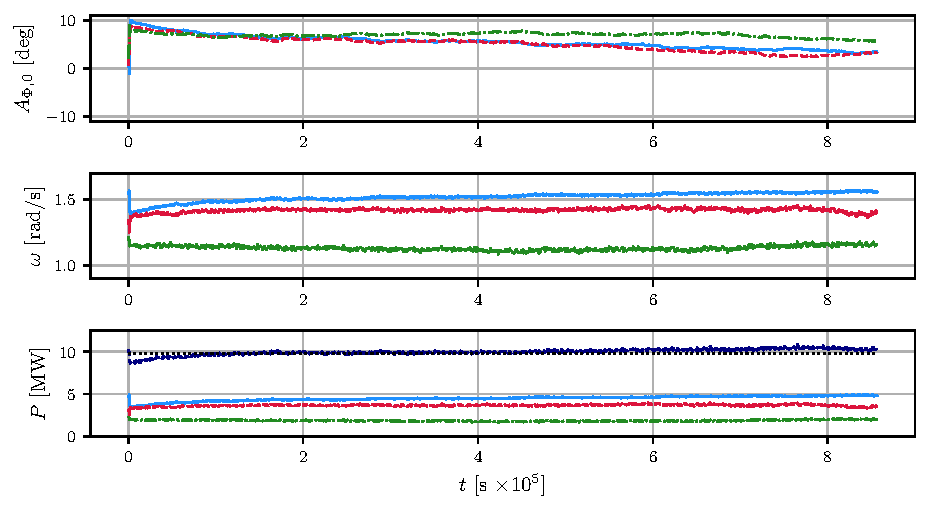
\includegraphics{behaviour_optimization/DIPC_training.pdf}
	\caption{\legendFive{Turbine 0}{Turbine 1}{Turbine 3}{Total}{Greedy.} Training of an agent controlling the amplitude of a sinusoidal variation of the pitch according to the helix approach. Only one environment shown. All values are a rolling average with a window of width $\SI{4359}{s}$. }
	\label{fig:dipc_big_training}
\end{figure}
The time series of the training of the agent with the large network as described in \autoref{ssec:dyn_description} is shown in \autoref{fig:dipc_big_training}. It shows the amplitude of the sinusoidal signal used to control the pitch angle, the angular velocity and the power of the three turbines as well as the combined power of the park. As a benchmark the mean power generated by a park controlled by the greedy controller is also given. In the beginning the agent performs considerably worse than the benchmark. It is also visible that the amplitude changes quickly at that point, while the changes afterwards is more gradual. The figure shows a strong correlation between increase in angular velocity and generated power for each turbine, which is to be expected since the generator torque is controlled by a greedy controller. The graph shows a steady increase in total power until about $\SI{7.5e5}{s}$. At this point the power begins to decline. Again, the agent cannot remain at a local optimum. This motivates a closer look at the results and also to apply domain knowledge to judge the results and not simply accept them as optimal.
\begin{figure}[h]
	\centering
	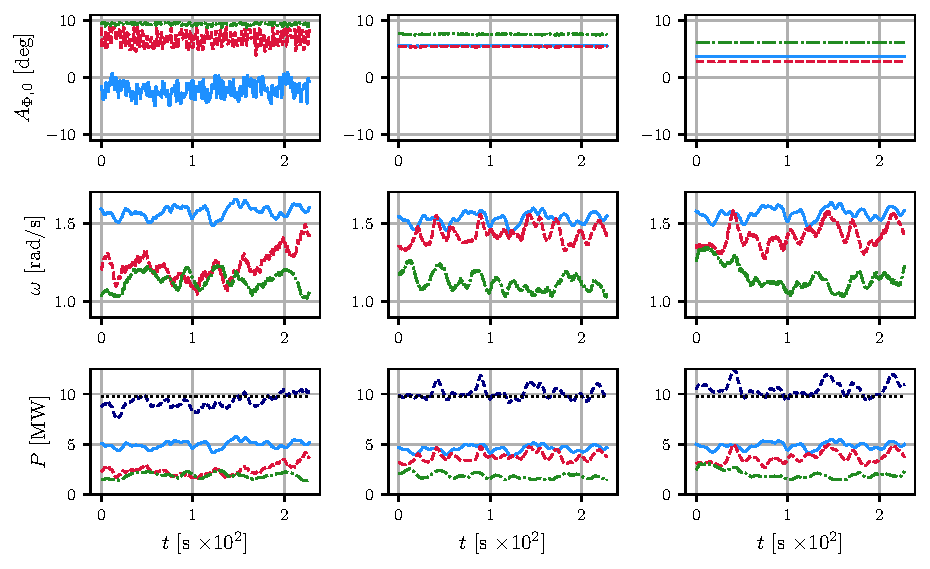
\includegraphics{behaviour_optimization/DIPC_eval.pdf}
	\caption{\legendFive{Turbine 0}{Turbine 1}{Turbine 3}{Total}{Greedy.} Control strategy at three points during training. Left at the beginning of the training, center after half of training time, right after the training is finalized.}
	\label{fig:dipc_big_strategies}
\end{figure}
A more detailed look into the evolution of the control strategy is offered by \autoref{fig:dipc_big_strategies}. It shows the same quantities as the figure before, for one flow through time. The results in the left column are obtained with the strategy after the first update, the results in the central column with the strategy after half of the training time and the left column displays the final strategy. It shows that the initial agent reacted to the fluctuating inputs of the network, whereas the agent in the final state sets constant amplitudes. The agent after half the training time still shows some reaction, most visible in the amplitude of the last turbines pitch. That this quantity evolves the slowest can be explained by the fact, that power production is the lowest at the last turbine. Therefore the same change in relative power or $C_P$ have a lower impact on the reward. Thus the control of the last turbine evolves the slowest. The figure also shows, that the power in the last turbine has changed little over the course of the training, which is also visible in \autoref{fig:dipc_big_training}. Instead, the increase in power can be attributed to the second turbine, while the first turbine actually decreased in power. The strategy obtained for the last turbine is highly questionable, since curtailment of the last turbine presumably offers no benefits. Therefore a greedy strategy, that is an amplitude of zero degrees would be expected. It cannot be ruled out that this strategy would emerge with longer training. However, the computed time to reach this strategy can roughly be estimated to be $\SI{5.75e5}{s}$, when taking the mean change in amplitude over the last $\SI{1e5}{s}$. Furthermore it shows that the amplitude of the pitch of the first and the second turbine are very similar, both about four degrees. This suggests that this a good balance between optimal $C_P$ and the effects allowing for a higher power production by the following turbine.
\subsection{Analysis of the control strategy}
\begin{table}[h]
	\centering
	\caption{Mean, relative difference in mean and relative difference in standard deviation of power and aerodynamic moment in comparison to the greedy controlled case.}
	\begin{tabular}{ccccccc}
	\toprule
	& \multicolumn{3}{c}{$P$}  & \multicolumn{3}{c}{$M_{aero}$ }\\ \cmidrule(rl){2-4} \cmidrule(rl){5-7}
	& mean & rel. mean & rel. std  & mean & rel. mean & rel. std \\ \midrule
	Total & $\SI{  10.4}{MW} $ & $\SI{ +6.75}{\%}$ & $\SI{ +4.78}{\%}$ &-&-&- \
	\\
	Turbine 0  & $\SI{  4.81}{MW} $ & $\SI{ -5.04}{\%}$ & $\SI{ -2.78}{\%}$ & $\SI{3.08e+03}{kNm} $ & $\SI{ -3.39}{\%}$ & $\SI{ -1.14}{\%}$ \\
	Turbine 1  & $\SI{  3.67}{MW} $ & $\SI{ +43.4}{\%}$ & $\SI{ +17.6}{\%}$ & $\SI{2.57e+03}{kNm} $ & $\SI{ +27.3}{\%}$ & $\SI{-0.331}{\%}$ \\
	Turbine 2  & $\SI{  1.97}{MW} $ & $\SI{ -8.95}{\%}$ & $\SI{ -12.2}{\%}$ & $\SI{1.7e+03}{kNm} $ & $\SI{ -6.08}{\%}$ & $\SI{ -1.53}{\%}$ \\
	\bottomrule
	\end{tabular}
	\label{tab:dipc_big_quants}
\end{table}
To also give more quantitative results, mean as well as relative changes in mean and standard deviation of comparison to the greedy controlled case of power and aerodynamic moment are given in \autoref{tab:dipc_big_quants}. It shows that the overall gain in power is almost seven percent. It also confirms the previous observation, that this gain in power is due to an increase in power production by the second turbine, which increase by more then 40 percent. Furthermore it strengthens the assumption that the strategy of the last turbine is not optimal, since power there actually decreased by almost nine percent. Since the strategy of both previous turbines is very similar, one could expect a similar increase in power as for the second turbine. Looking beyond a simple increase in power production, quality of generated power and turbine loads are of very high importance. One measure of quality of power is low fluctuations, which is why the standard deviation of power is also given in \autoref{tab:dipc_big_quants}. It shows, that they increase in total power produced, due to a big increase in the fluctuations at the second turbine. The second aspect is the loads of the turbine, which is also a very active area of research. Therefore the analysis of loads will not be thorough, it is only pointed out, that aerodynamic torque have decreased at the first turbine and that the fluctuations have decreased at all the turbines. Therefore, like power production, the aerodynamic torque is more evenly distributed amongst the turbines, which likely has a beneficial influence on turbine lifetime. The influence on the thrust force were already assessed in \cite{frederik_helix_2020}, where only small differences were found.
\begin{figure}[h]
	\centering
	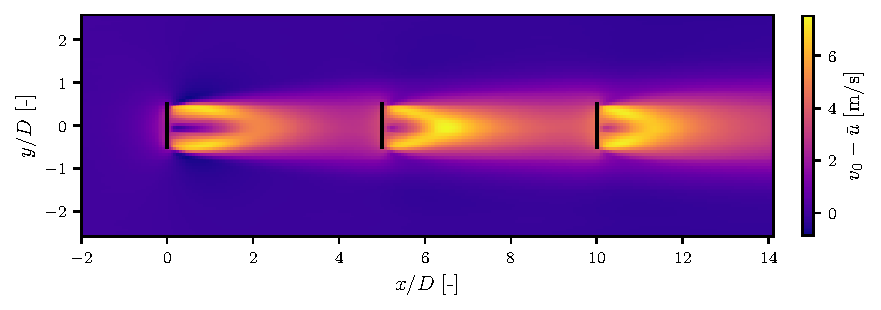
\includegraphics{behaviour_optimization/DIPC_velocity.pdf}
	\caption{{\color{black} \rule[3pt]{22pt}{1pt} Turbine.} Mean velocity deficit compared to mean wind speed with optimized helix control.}
	\label{fig:dipc_big_vel}
\end{figure}

\begin{figure}[h]
	\centering
	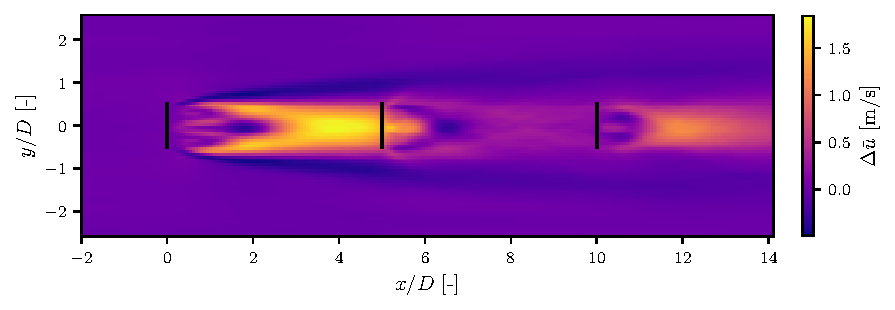
\includegraphics{behaviour_optimization/DIPC_velocity_difference.pdf}
	\caption{{\color{black} \rule[3pt]{22pt}{1pt} Turbine.} Difference in mean velocity between optimized helix control and greedy control.}
	\label{fig:dipc_big_vel_dif}
\end{figure}
To assess the causes for the increase in power, \autoref{fig:dipc_big_vel} and \autoref{fig:dipc_big_vel_dif} show the velocity deficit in comparison to the mean wind speed and the difference in velocity in comparison to the greedy control case. As expected, a wake deficit of up to $\SI{7}{m/s}$ is visible after each turbine. Differences arise in the form of the deficit. The deficit is strongest at the tips of the blades in all cases, but at the second and the third turbine these minima meet in the center of the wake shortly behind the turbine, while they stay separated behind the first turbine. Comparing the fluid field in front of the turbine shows that the deficit in front of the third turbine is larger than in front of the second turbine. While some of the lower power production probably has to be attributed to the suboptimal control strategy, power production of the third turbine can probably not reach the amount of the second turbine since the inflow velocity is smaller. In the comparison to the greedy control case, the increased speed in the wake is brightly visible, with difference of $\SI{1.5}{m/s}$ at the core of the wake. One can also see an area of lower mean speed on the edge of the deficit. This means that the wake in the helix approach is more spread out, which is the motivation behind this approach. Behind the second turbine wind speeds are also higher, but the difference is not as big as in the first turbines wake. This is an important observation in the general behaviour of the helix approach, since Frederik et al. only considered two turbines in their study \cite{frederik_helix_2020}. If the increase in velocity can not be found after the second turbine, application to a find warm is not as beneficial as suggested by the initial study. The wake after the third turbine has again a higher velocity than in the greedy case, which again points to the fact, that more power could be generated by the third turbine.  
\begin{figure}[h]
	\centering
	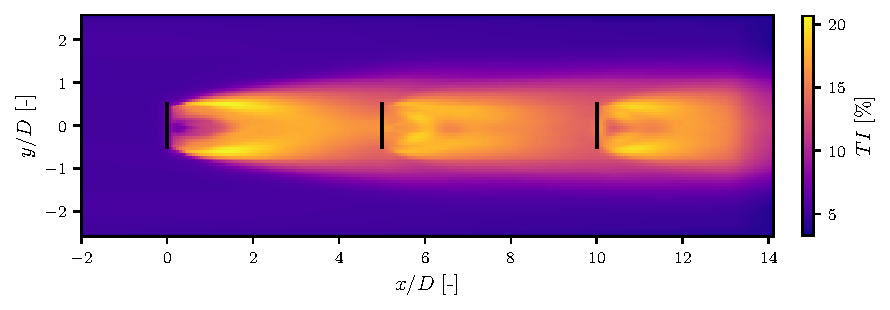
\includegraphics{behaviour_optimization/DIPC_turbulence_intensity.pdf}
	\caption{{\color{black} \rule[3pt]{22pt}{1pt} Turbine.} Turbulence intensity of optimized helix control.}
	\label{fig:dipc_big_ti}
\end{figure}
\begin{figure}[h]
	\centering
	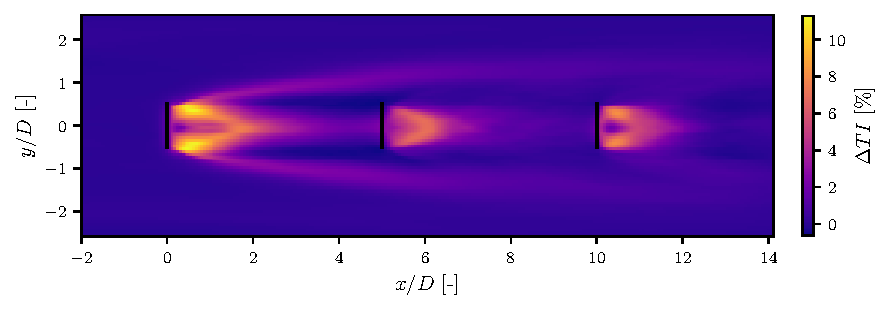
\includegraphics{behaviour_optimization/DIPC_ti_difference.pdf}
	\caption{{\color{black} \rule[3pt]{22pt}{1pt} Turbine.} Difference in turbulence intensity between optimized helix control and greedy control.}
	\label{fig:dipc_big_ti_dif}
\end{figure}
The previous figures showed, that the second turbine caused a bigger wake deficit compared to inflow velocity than if it was greedy controlled. This is not the case after the first turbine, where the deficit is significantly lower. A possible explanation for this can be found in the secondary statistics of the fluid, that is its fluctuations. Therefore \autoref{fig:dipc_big_ti} shows the turbulence intensity of the helix control case and \autoref{fig:dipc_big_ti_dif} the difference of the helix control case to the greedy control case. The first figure shows that the turbulence intensity is up to four times higher in the wake. It also shows, that areas, that have a high velocity deficit, are surround by an area of high turbulence intensity. This is expected, since these are areas of high velocity gradients. Another observation that can be made is that the area with increased turbulence intensity grows in diameter up to about half a turbine distance after the second turbine and stays constant after that. A high turbulence intensity at the edges of the wake is desirable since this increases mixing of the undisturbed fluid with high momentum and fluid in the wake with less momentum. The comparison to the greedy controller shows, that this is achieved by the helix approach.\\
\begin{figure}[h]
	\centering
	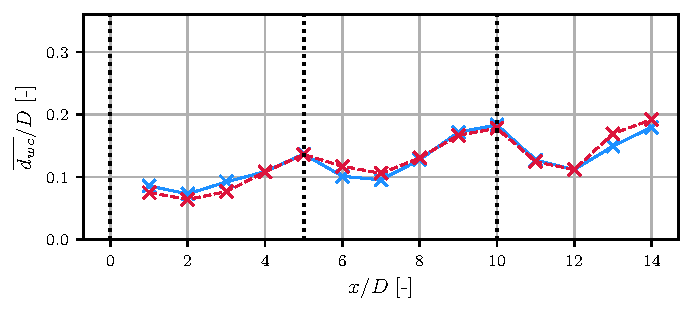
\includegraphics{behaviour_optimization/centers.pdf}
	\caption{\legendTwo{Helix}{Greedy}{\color{black}\rule[3pt]{1pt}{1pt} \rule[3pt]{1pt}{1pt} \rule[3pt]{1pt}{1pt} \rule[3pt]{1pt}{1pt} \rule[3pt]{1pt}{1pt} \rule[3pt]{1pt}{1pt}} Turbines. Mean distance of wake center to plane center. Crosses mark the location of the planes in which the wake center is calculated.}
	\label{fig:centers}
\end{figure}
In order to analyze the influence of the helix approach on the dynamics of the wake, the wake centers were calculated using the samwich toolbox \footnote{\url{https://github.com/ewquon/waketracking}} provided by NREL. It contains different methodologies to determine the wake center. In this work the wake center is defined as the center of a least-sqeare fit of a Gaussian bell curve to the velocity deficit. \autoref{fig:centers} shows the distance of the wake center $d_{wc}$ to the center of the cross stream plane averaged over 100 snapshots of the fluid field at 14 planes downstream of the first turbine with a distance of a turbine diameter. It shows, that the wake is steered further away from the center after the first turbine, while this is not the case after the second turbine, where greedy and helix control lay on top of each other. After the third turbine the helix control increases the mean wake distance again. Areas, where $\overline{d_{wc}}$ is larger correspond to areas with lower mean wake deficit, which shows, that the wake is not expanded in comparison to the greedy control case, but skewed away from the center. This also explains, why a band of high turbulence intensity was visible in \autoref{fig:dipc_big_ti_dif}. This is the area only reached by the wake of the helix control case. Remarkably, the helix approach is not able to the skew the wake after the second turbine. This is most likely why the third turbine cannot increase its power production. Several aspects can contribute to this. First, the increased turbulence intensity in comparison to the inflow of the first turbine likely diffuses the tangential momentum added by the blades. Furthermore, it is questionable, whether the frequency at which the blade pitch is altered is appropriate at the second turbine. Frederik et al. showed that the wake deficit is sensitive to the Strouhal number in \cite{frederik_helix_2020}. Assuming a velocity deficit of $\SI{3}{m/s}$, the Strouhal number would increase from $\SI{0.25}{}$ to $\SI{0.35}{}$, which, according to Frederik et al., is still close to the minimal wake loss. Thus this is a possible point for future optimization, but does not account for the entire effect. However, the decreased velocity also has an effect on tangential forces exerted on the wake, since the relative velocity at the blade and the angle of attack change. Both these changes decrease the tangential force. \\
The training data showed, that the training requires a lot of computational time and that optimization is slow. However, the results did continually improve for most of the training, but, as was seen in the parameter studies as well, optimal behaviour is lost again after more training. Therefore, results of training can not be guaranteed to be optimal. The analysis of the optimized helix control showed, that due to the wake steering an increase in power production by the second turbine is possible, with little decrease in production of the first turbine. However, it also showed, that steering of the second wake was not achieved and therefore benefits for the third turbine are small, in this case even resulted in a decrease of power. Further testing of this strategy is required, for example in sheared inflow and in a park with more turbines.
